
\section{Barrier Certificate Search for Second Order Robot Slide System}\label{sec:sos_2ndorder_error}

To complete the construction of barrier certificates with SOSTOOLS for the robot slide movement parallel to the construction of \glspl{cbf} in \autoref{chap:cbf_1d_static}, and in order to test SOSTOOLS on a system of a higher state space dimension, finally a barrier certificate is found for the second order model of the robot slide position from \autoref{subsec:model_2d}. 

As for the first order model in \autoref{sec:sos_search_1storder}, safety is validated for the closed loop system using a linear position controller. The system is tested for safety compliance using the same controller gains as presented in \autoref{sec:K_Nbar_1D_2ndorder} with proportional gain $\mathbf{K}=[K_1\,\,\,\,K_2]=[5.173\,\,\,\,0.214]$ and unity gain between reference and position secured by $\bar{\mathbf{N}}=K_1+1=6.173$. The closed-loop second order system with $x_1=$ position and $x_2=$ velocity of the end-effector, is recapitulated as
\begin{equation}
\dot{\mathbf{x}} = 
\dot{\begin{bmatrix}
	x_1\\x_2
	\end{bmatrix}} = 
\begin{bmatrix}
0 & 1\\
-\omega_n^2  & -2\zeta \omega_n  
\end{bmatrix}
\begin{bmatrix}
x_1\\x_2
\end{bmatrix} + 
\begin{bmatrix}
0\\\omega_n^2
\end{bmatrix}\left(\bar{\mathbf{N}}x_\text{ref}-
\underbrace{\begin{bmatrix}
K_1 & K_2
\end{bmatrix}}_{\mathbf{K}}
\begin{bmatrix}
x_1\\x_2
\end{bmatrix}\right),
 \quad \text{with}
\begin{matrix*}[l]
\phantom{\zeta}\omega_n = 17 \,\text{rad/s}\\  \phantom{\omega_n}\zeta = 0.55
\end{matrix*}
\label{eq:sos_2ndorder}
\end{equation}
%where again the matrix $\bar{\mathbf{N}}$ ensures unity gain between the position and its reference, which means that $\bar{\mathbf{N}}=K_1+1$. Now the position error is 
From the analysis in \autoref{sec:sos_1storder_error} it is found that a coordinate shift from absolute to relative positions in the form of the position error proves the more efficient method to validate system safety for a wide range of references. Using the position error $x_\text{err,1}$ as the free variable and letting $x_\text{err,2}$ signify the rate of change of the error, the dynamics of the error state can be expressed as
\begin{align*}
x_\text{err,1}&=x_\text{ref}-x_1\\
\dot{x}_\text{err,1} &= -\dot{x}_1 \,=-x_2=x_\text{err,2}\\
\ddot{x}_\text{err,1} &= \dot{x}_\text{err,2} = -\dot{x}_2 = \omega_n^2 x_1 +2\zeta\omega_n x_2 - \omega_n^2(\bar{\mathbf{N}}x_\text{ref}-(K_1x_1+K_2 x_2))\nonumber\\
& \phantom{= -\ddot{x}_\text{err,1} = \dot{x}_2. } = (2\zeta\omega_n +K_2)x_2 -\omega_n^2(K_1+1)(x_\text{ref}-x_1)\nonumber\\
& \phantom{= -\ddot{x}_\text{err,1} = \dot{x}_2. } = -(2\zeta\omega_n +K_2){x}_\text{err,2} - \omega_n^2(K_1+1)x_\text{err,1}
%- 5.173\dot{x}_1(t)  -  0.214\dot{x}_2(t) &= -5.173x_2 -0.214(- \omega_n^2 x_1 - 2\zeta \omega_n x_2 + \omega_n^2 x_\text{err} )\nonumber\\
%&= (0.214\cdot2\zeta \omega_n - 5.173)x_2 + 0.214\omega_n^2\underbrace{(x_1-x_\text{err})}_{\textcolor{red}{x_\text{ref} ???}}
\end{align*}
which can be compressed to standard state space form as
\begin{equation}
\dot{\mathbf{x}}_\text{err}= 
\dot{\begin{bmatrix}
{x}_\text{err,1} \\ 
{x}_\text{err,2}
\end{bmatrix}} =
\begin{bmatrix}
0 & 1 \\
-\omega_n^2(K_1+1) & -(2\zeta\omega_n +K_2)
\end{bmatrix}
\begin{bmatrix}
x_\text{err,1} \\ {x}_\text{err,2}
\end{bmatrix}
\label{eq:sos_2ndorder_error}
\end{equation}

\subsubsection{Relating the Error State Space Sets to the Sets for Absolute Position}

\vspace{-2mm}
The relation between the state space system of absolute positions in \autoref{eq:sos_2ndorder} and relative positions in \autoref{eq:sos_2ndorder_error} is equivalent to the relation presented in \autoref{sec:sos_1storder_error}.
Again, as seen in \autoref{fig:sos_slide}, the unsafe positions are positions in the upper end of the interval of positions in the set $\mathcal{X}$, which means that for references given outside the unsafe set, the system can only be unsafe if the robot end-effector position is above the reference, corresponding to a negative error. This is illustrated in \autoref{fig:sos_delta_error_2ndorder} with an overshoot, although the system presented should  not overshoot due to the placement of real poles (in -40 and -50, see \autoref{eq:K_2}). When the error can be guaranteed to stay above a value -$\delta_\text{err}$, this is equivalent to guaranteeing that the end-effector position will never be more than the distance $\delta_\text{err}$ above the reference which in turn means that the system is safe for all references with a minimum distance $\delta_\text{err}$ to the unsafe region. This is illustrated in \autoref{fig:sos_errorref_1d_new_2ndorder}.

\vspace{-2mm}
\begin{figure}[htbp]
	\centering
	\subbottom[]{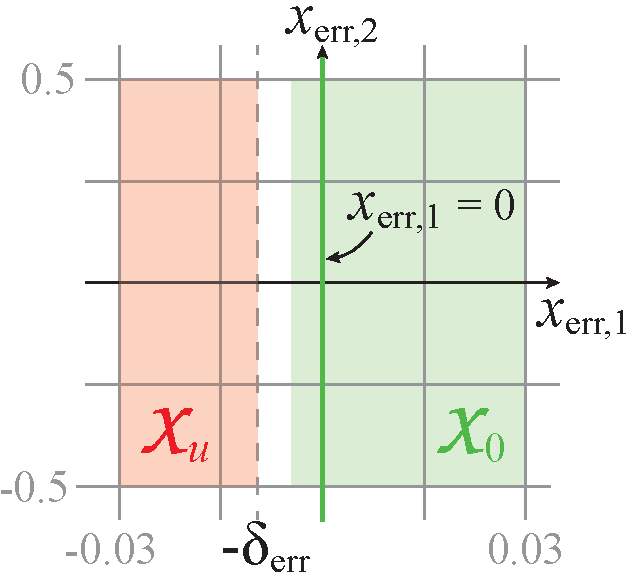
\includegraphics[width=0.3\textwidth]{sos_error_2d_2ndorder.pdf}\label{fig:sos_error_2d_2ndorder}}%
	\hspace{3mm}
	\subbottom[]{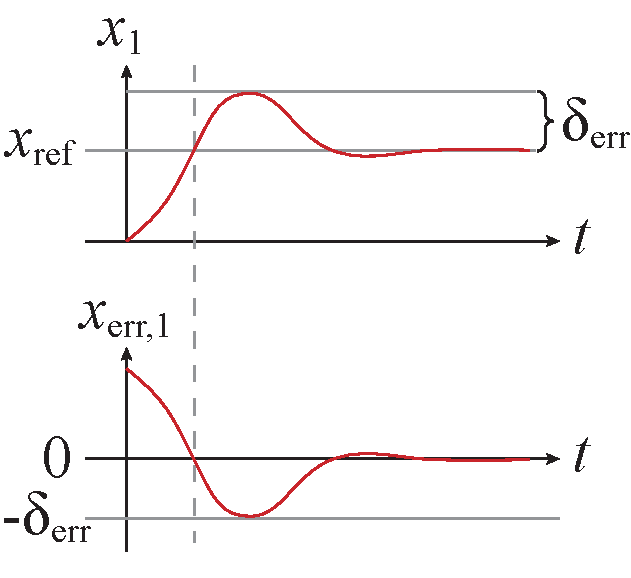
\includegraphics[width=0.3\textwidth]{sos_delta_error_2ndorder.pdf}\label{fig:sos_delta_error_2ndorder}}%
	\hspace{3mm}
	\subbottom[]{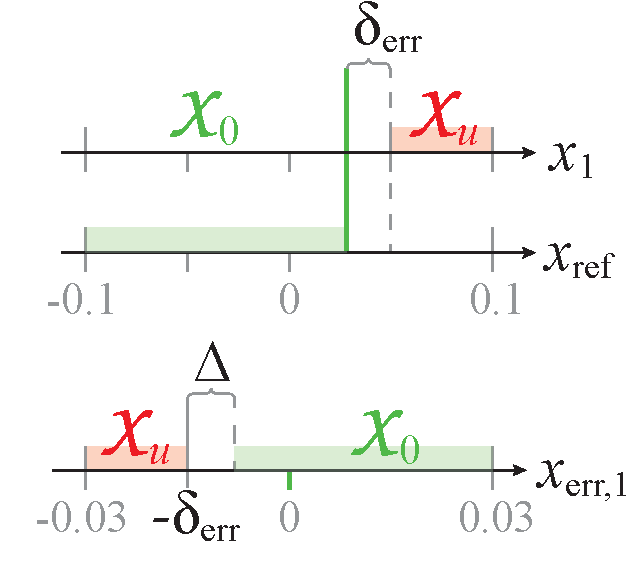
\includegraphics[width=0.3\textwidth]{sos_errorref_1d_new_2ndorder.pdf}\label{fig:sos_errorref_1d_new_2ndorder}}%
	\caption{With references given outside the unsafe region, system safety can be guaranteed if the error is certified to stay above the value $-\delta_\text{err}$. When this is the case, system safety is guaranteed for all references up to a safety distance of $\delta_\text{err}$ from the unsafe set.}
	\label{fig:sets_error_2ndorder}
\end{figure}

Equivalent to the first order system, the model in \autoref{eq:sos_2ndorder} is tested and known to be valid for small steps of approximately 5\,mm, and again the set $\mathcal{X}$ to be considered is chosen to $\pm 3$\,cm.
For the second order system, the sets $\mathcal{X}$, $\mathcal{X}_u$ and $\mathcal{X}_0$ must also be specified for the velocity dimension. As the rate of change of the error is related to the end-effector velocity by a factor -1, the considered interval of velocities is chosen as the upper limits for the robot slide velocity of $\pm 0.5$\,m/s \textcolor{red}{REFRERENCE TIL SLIDE M\AA LING}. This is visualized in \autoref{fig:sos_error_2d_2ndorder}, and gives the set definitions for the second order error state system:
\vspace{-2mm}
\begin{itemize}
\itemsep-0.7mm
\item The set considered is well over the usual reference step size of 5\,mm, and the the upper bound on the velocity  considered is the physical limits of the system from \textcolor{red}{REFRERENCE TIL SLIDE M\AA LING}, $\mathcal{X}=\{x_\text{err,1}\in[-0.03,0.03], \,\,\, x_\text{err,2}\in[-0.5,0.5] \}$.
\item The unsafe set includes relative positions below -$\delta_\text{err}$, $\mathcal{X}_u=\{x_\text{err,1}\in[-0.03,-\delta_\text{err}],\,\,\, x_\text{err,2}\in[-0.5,0.5] \}$.
\item The safe set is a distance $\Delta$ from the unsafe position, where $\Delta<\delta_\text{err}$ such that the safe set will include $x_\text{err,1}=0$, $\mathcal{X}_0=\{x_\text{err,1}\in[-\delta_\text{err}+\Delta,0.03], \,\,\, x_\text{err,2}\in[-0.5,0.5] \}$.
\end{itemize}

If a valid solution can be found, it will certify that that steps in positive direction (upwards) of 3\,cm and system velocities up to $\pm 0.5$\,m/s are acceptable, and will never yield an error below -$\delta_\text{err}$, which means that references can safely be given as long as they have a distance of at least $\delta_\text{err}$ to the unsafe positions, hence certifying safety of the system:
\vspace{-2mm}
\begin{itemize}
\itemsep-0.7mm
\item The positions considered are as described in \autoref{fig:sos_slide}, and the velocity is bounded by the physical limits of the system from \textcolor{red}{REFRERENCE TIL SLIDE M\AA LING}, $\mathcal{X}=\{x_1\in[-0.1,0.1],\,\,\, x_2\in[-0.5,0.5] \}$.
\item The unsafe positions are also seen in \autoref{fig:sos_slide}, $\mathcal{X}_u=\{x_1\in[0.05,0.1],\,\,\, x_2\in[-0.5,0.5] \}$.
\item The safe set for the reference is $\mathcal{X}_0=\{x_\text{ref}\in[-0.1,0.05-\delta_\text{err}]$ ensuring that $\mathcal{X}_0\subseteq\mathcal{X}\setminus\mathcal{X}_u$.
\end{itemize}

%As for the first order system, the unsafe set is $\mathcal{X}_u=\{x_1\in[0.05,0.1] \}$, and it is assumed that references are never given in the unsafe set (or outside the physical limits of the slide position). Hence it is again the goal to limit the position error in negative direction (tool position above reference), while the velocity of the error obviously has the same physical limits as the velocity of the robot tool, i.e. a maximum velocity of . This means that the sets are defined as $\mathcal{X}=\{x_\text{err,1}\in[-0.03,0.03], x_\text{err,2}\in[-1,1] \}$, the unsafe set $\mathcal{X}_u=\{x_\text{err,1}\in[-0.03,-\delta_\text{err}], x_\text{err,2}\in[-1,1] \}$ and the safe set $\mathcal{X}_0=\{x_\text{err,1}\in[-\delta_\text{err} +\Delta,0.03], x_\text{err,2}\in[-1,1] \}$, see \autoref{fig:sos_error_2d_2ndorder}, and it is again desired to find as small a value $\delta_\text{err}$ as possible, thus guaranteeing system safety for references until a minimum distance $\delta_\text{err}$ from the region of unsafe positions, see \autoref{fig:sos_error_1d_2ndorder} and \ref{fig:sos_errorref_1d_2ndorder}.

\subsubsection{Results and Conclusions}

\vspace{-2mm}
The parameters $\bar{\epsilon}$, $\Delta$, $\delta_\text{err}$, and the degree of the \gls{sos} polynomials $q_j$ and the polynomial $B(x)$, are tweaked to find the smallest possible value of $\delta_\text{err}$ yielding a valid solution.
The MATLAB implementation of this certificate can be found in appendix \ref{app:sos_errorstate_secondorder} and in \autoref{app:cd} under the path \texttt{matlab\_scripts/}\texttt{sostools/} \texttt{2ndorder\_error.m}.
The findings conform with the conclusions presented in \autoref{tab:sostools_varying_param} and \autoref{tab:sostools_varying_param_error}. The choice of the parameter values is presented in \autoref{tab:sostools_choice_error2} and the  barrier certificate is plotted in \autoref{fig:1D_2ndordersys_error_B4_q1_e5-2_d5-3_8mm}.

%Again, the same parameters as in \autoref{sec:sos_1storder_references} and \ref{sec:sos_1storder_error} are varied, and the same conclusions are drawn i.e. in general decreasing either  $\Delta$, $\bar{\epsilon}$ or deg$(q)$ decreases the residual norm. With  $\textbf{K}=[5.173  \,\,\,\,  0.214]$ as determined in \autoref{eq:K_2}, solutions can be found to the problem for $\delta_\text{err}=8$\,mm and above, again signifying a verification that the system is safe for references given at a distance of least 8\,mm from the unsafe area.

\begin{table}[htbp]
	\begin{tabularx}{\textwidth}{l X}
		\rowcolor{HeaderBlue}
		\textbf{Choice} & \textbf{Reason}\\
		deg$(B)=$ [0:4] & %Compared to the first order system increasing the degrees of the barrier function and the \gls{sos} polynomials  more clearly causes a scaling of the functional values, while the curves are close to identical in shape on the sets. 
		The residual norm of the solution is growing when the polynomial degrees are increased, thus the smallest degree of $B(x)$ yielding a solution is chosen. 
		%Numerical problems are reported for all three solutions as for almost all solutions found, however, numerical errors are only indicated for the two lowest-order polynomials plotted in .
		\\
		\rowcolor{textBlue}
		deg$(q_j)=$ [0:1] & Decreasing the degree of the \gls{sos} polynomials decreases the residual norm of the solution, hence the degree is chosen as low as possible.\\
		$\bar{\epsilon}=5e$-2 & The value of $\bar{\epsilon}$ is chosen from the solution yielding the best compromise between small residual norm and feasibility ratio close to 1. \\
		\rowcolor{textBlue}
		$\Delta=5e$-3 & The smallest possible value of $\Delta$ yielding a solution for the chosen $\delta_\text{err}$.\\
		$\textbf{K}=[5.173  \,\,\,\,  0.214]$ & Choice of closed loop system with real poles from \autoref{eq:K_2}.\\
		\rowcolor{textBlue}
		$\delta_\text{err}=8e$-3 & No solutions could be found for $\delta_\text{err}<8$\,mm.
	\end{tabularx}
	\caption{Chosen value for each of the parameters. The barrier certificate is plotted in \autoref{fig:1D_2ndordersys_error_B4_q1_e5-2_d5-3_8mm}.}
	\label{tab:sostools_choice_error2}
\end{table}

\begin{figure}[H]
	\centering
	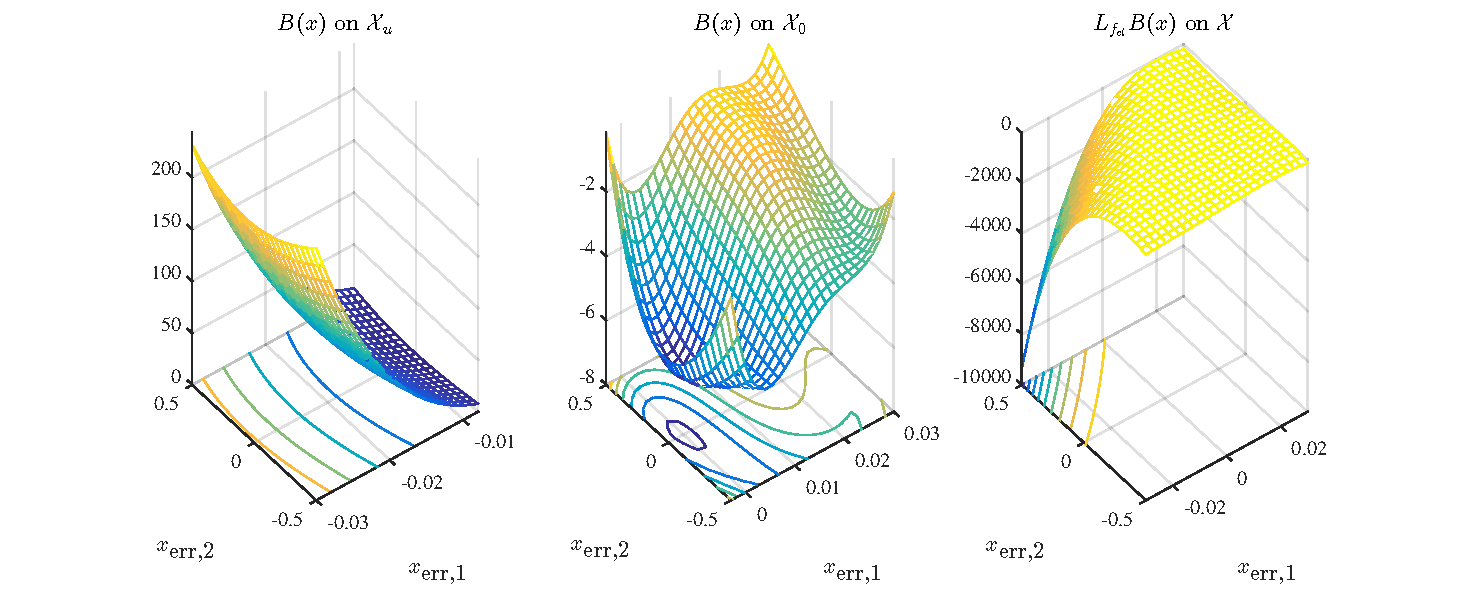
\includegraphics[width=\textwidth]{1D_2ndordersys_error_B4_q1_e5-2_d5-3_8mm.pdf}
	\caption{Barrier certificate of degree [0:4], all \gls{sos} polynomials of degree [0:1], $\bar{\epsilon}=5$e-2, $\Delta=5$\,mm, $\delta_\text{err}=8$\,mm and gain $\textbf{K}=[5.173  \,\,\,\,  0.214]$ gives \texttt{feasratio=1.0176} and \texttt{Residual norm=3.2e-6}.}
	\label{fig:1D_2ndordersys_error_B4_q1_e5-2_d5-3_8mm}
\end{figure}

%\begin{figure}[H]
%	\centering
%	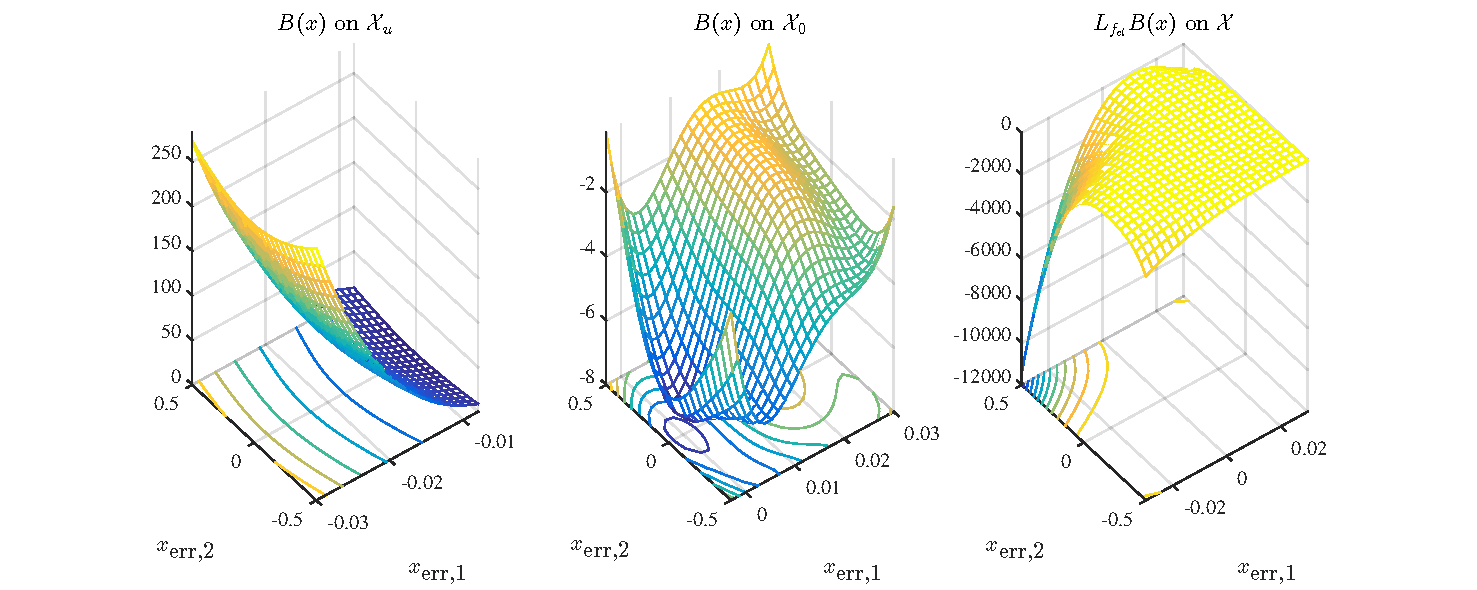
\includegraphics[width=\textwidth]{1D_2ndordersys_error_B6_q2_e5-2_d5-3_8mm.pdf}
%	\caption{Barrier certificate of degree [0:6], all \gls{sos} polynomials of degree [0:2], $\bar{\epsilon}=5$e-2, $\Delta=5$\,mm and $\delta_\text{err}=8$\,mm gives \texttt{feasratio=0.9500} and \texttt{Residual norm=1.8e-5}.}
%	\label{fig:1D_2ndordersys_error_B6_q2_e5-2_d5-3_8mm}
%\end{figure}

%\begin{figure}[H]
%	\centering
%	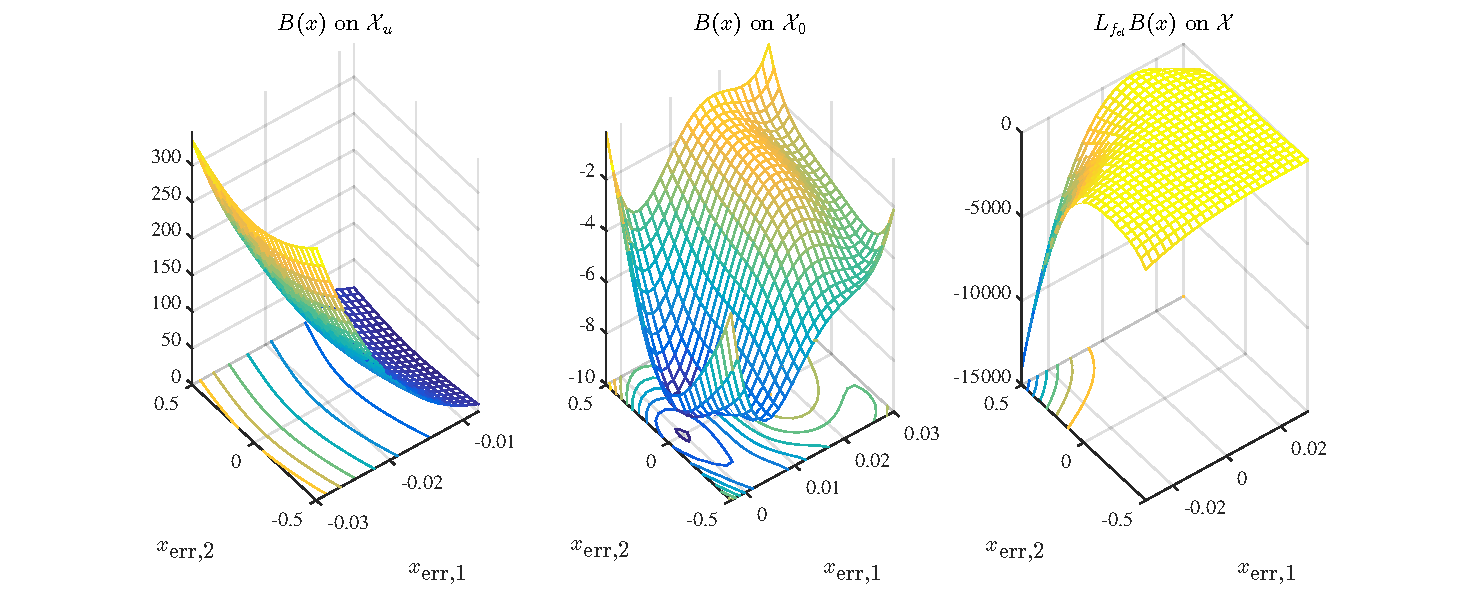
\includegraphics[width=\textwidth]{1D_2ndordersys_error_B8_q3_e5-2_d5-3_8mm.pdf}
%	\caption{Barrier certificate of degree [0:8], all \gls{sos} polynomials of degree [0:3], $\bar{\epsilon}=5$e-2, $\Delta=5$\,mm and $\delta_\text{err}=8$\,mm gives \texttt{feasratio=0.9882} and \texttt{Residual norm=4.5e-5}.}
%	\label{fig:1D_2ndordersys_error_B8_q3_e5-2_d5-3_8mm}
%\end{figure}

%Three examples of solutions are seen in \autoref{fig:1D_2ndordersys_error_B4_q1_e5-2_d5-3_8mm}, \ref{fig:1D_2ndordersys_error_B6_q2_e5-2_d5-3_8mm} and \ref{fig:1D_2ndordersys_error_B8_q3_e5-2_d5-3_8mm} with $\delta_\text{err}=8$\,mm and with a minimum value in the unsafe set $\bar{\epsilon}=5$e-2. 
%\autoref{fig:1D_2ndordersys_error_B4_q1_e5-2_d5-3_8mm} and \ref{fig:1D_2ndordersys_error_B6_q2_e5-2_d5-3_8mm}, but not for the solution plotted in \autoref{fig:1D_2ndordersys_error_B8_q3_e5-2_d5-3_8mm}.

%From \autoref{eq:K_2}
%\begin{flalign}
%	\mathbf{K} = \texttt{acker(A,B,C,D,[-40 -50])} = \begin{bmatrix}
%		5.173  &  0.214
%	\end{bmatrix}
%\end{flalign}

%From \autoref{eq:Nbar_2}
%\begin{flalign}
%	\bar{\mathbf{N}} = - \left( \mathbf{C}\,\mathbf{A}_{cl}^{-1}\,\mathbf{B} \right)^{-1} =  - \left( \mathbf{C}\,(\mathbf{A}-\mathbf{B}\,\mathbf{K})^{-1}\,\mathbf{B} \right)^{-1} = 6.173
%\end{flalign}

It is seen from \autoref{fig:1D_2ndordersys_error_B4_q1_e5-2_d5-3_8mm} that the barrier certificate is positive on the unsafe region for positions below -8\,mm, i.e. $\mathcal{X}_u=\{\mathbf{x}_\text{err}\in[-0.03,0.008]\times[-0.5,0.5]\}$, and nonpositive on the safe region $\mathcal{X}_0=\{\mathbf{x}_\text{err}\in[-0.005,0.03]\times[-0.5,0.5]\}$, and that its Lie derivative is nonpositive on the entire set $\mathcal{X}=\{\mathbf{x}_\text{err}\in[-0.03,0.03]\times[-0.5,0.5]\}$, confirming that it is a valid barrier certificate for the system in \autoref{eq:sos_2ndorder_error} in accordance with \autoref{def:barrier_certificate}.

Relating the relative position to the absolute positions, this certificate guarantees safety for the system in \autoref{eq:sos_2ndorder} for refereces up until a minimum distance of 8\,mm from the unsafe positions $\{x_1\in[0.05,0.1] \}$ (see \autoref{fig:sos_slide}), i.e. system safety is guaranteed for references in the interval $\mathcal{X}_0=\{x_\text{ref}\in[-0.1,0.042] \}$. Comparing this result to the conclusion drawn for the first order system in \autoref{sec:sos_1storder_error}, it is seen that for the second order system safety is certified for references that are 1\,mm closer to the unsafe set. This is attributed coincidence in the combination of tested parameter values, and it is thus expected that safety can be guaranteed for the first order system for references closer to the unsafe set than 9\,mm using a different combination of parameter values.



\section{Conclusion on the Use of SOSTOOLS}\label{sec:sos_conclusion}
